\documentclass{article}

\usepackage{amsmath, mathrsfs, amssymb, stmaryrd, cancel, relsize,tikz,amsthm,comment,enumerate}

\theoremstyle{definition}
\newtheorem{Q}{Question}
\newtheorem{definition}{Definition}

\newcommand{\tvs}{\textvisiblespace}
\newcommand{\ra}{\rightarrow}
\newcommand{\la}{\leftarrow}
\newcommand{\co}{\mathbf{code}}
\newcommand{\NP}{\mathbf{NP}}
\newcommand{\bbN}{\mathbb{N}}
\newcommand{\bbR}{\mathbb{R}}
\newcommand{\SAT}{\mathsf{PSAT}}

%\includecomment{comment}


\title{ITCS 532 Foundations of Computer Science\\
Week 8 Quiz}
\author{Rob Egrot}
\date{}

\begin{document}
\maketitle

\begin{Q}
Let $\Sigma = \{a,b\}$. Given $n\in \bbN$ let e.g. $a^n$ be the string that is the $a$ symbol $n$ times. For example, $b^3 = bbb$. Let $L=\{a^nb^n:n\in \bbN\setminus\{0\}\}$. Design a Turing machine that decides $L$. Express this machine as a state change diagram.  
\end{Q}
\begin{comment}
\textbf{Solution}
Undefined transitions can be considered to lead to the reject state. The idea is that $a$ is expected as the first symbol. If the 1st symbol is not $a$ then the machine rejects immediately. If it is $a$ then the machine erases it then looks for the last symbol, which it expects to be a $b$. If it is not a $b$ then the machine rejects. If it is a $b$ then the machine erases it and looks for the first non-blank symbol, which it expects to be $a$. If it is $a$ it erases it then looks for the last symbol, which it expects to be $b$, etc. This process of erasing the first $a$ and the last $b$ repeats. If the string has the right form then the machine will end up erasing the whole input and accepting. If it is not the right form then it will not see an $a$ or $b$ at some point when it expects to, and so will reject. Note that this algorithm could be made more efficient at the cost of a more complicated Turing machine.
\begin{center}
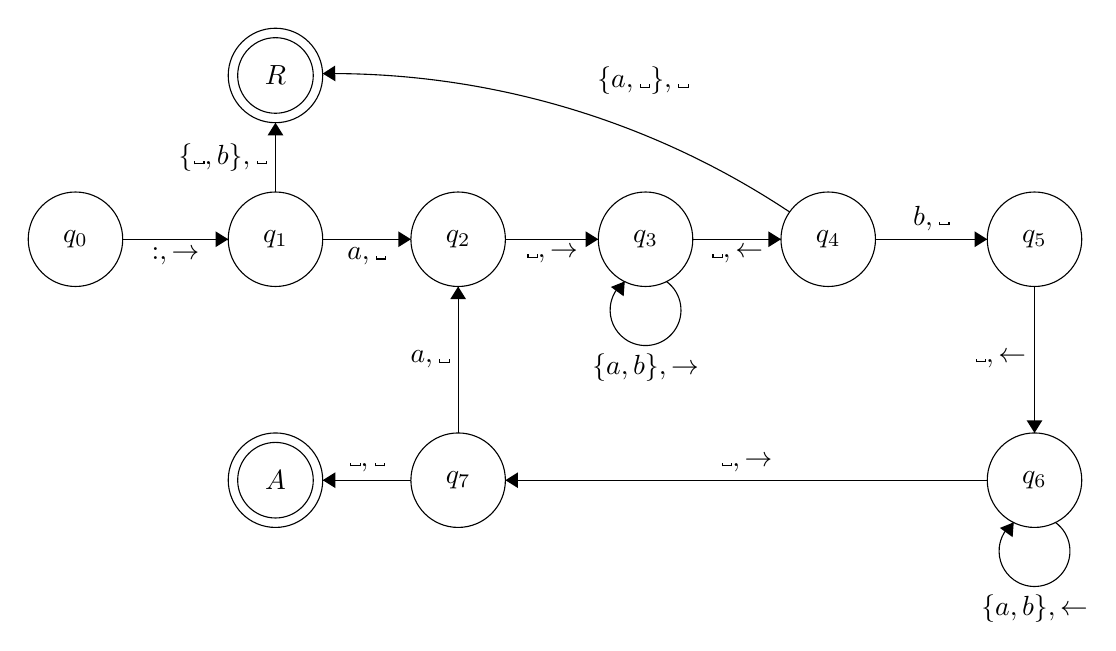
\begin{tikzpicture}[scale=0.2]
\tikzstyle{every node}+=[inner sep=0pt]
\draw [black] (7.5,-14) circle (3);
\draw (7.5,-14) node {$q_0$};
\draw [black] (20.2,-14) circle (3);
\draw (20.2,-14) node {$q_1$};
\draw [black] (20.2,-3.6) circle (3);
\draw (20.2,-3.6) node {$R$};
\draw [black] (20.2,-3.6) circle (2.4);
\draw [black] (31.8,-14) circle (3);
\draw (31.8,-14) node {$q_2$};
\draw [black] (43.7,-14) circle (3);
\draw (43.7,-14) node {$q_3$};
\draw [black] (55.3,-14) circle (3);
\draw (55.3,-14) node {$q_4$};
\draw [black] (68.4,-14) circle (3);
\draw (68.4,-14) node {$q_5$};
\draw [black] (68.4,-29.3) circle (3);
\draw (68.4,-29.3) node {$q_6$};
\draw [black] (20.2,-29.3) circle (3);
\draw (20.2,-29.3) node {$A$};
\draw [black] (20.2,-29.3) circle (2.4);
\draw [black] (31.8,-29.3) circle (3);
\draw (31.8,-29.3) node {$q_7$};
\draw [black] (10.5,-14) -- (17.2,-14);
\fill [black] (17.2,-14) -- (16.4,-13.5) -- (16.4,-14.5);
\draw (13.85,-14.5) node [below] {$:,\rightarrow$};
\draw [black] (20.2,-11) -- (20.2,-6.6);
\fill [black] (20.2,-6.6) -- (19.7,-7.4) -- (20.7,-7.4);
\draw (19.7,-8.8) node [left] {$\{\tvs,b\},\tvs$};
\draw [black] (23.2,-14) -- (28.8,-14);
\fill [black] (28.8,-14) -- (28,-13.5) -- (28,-14.5);
\draw (26,-14.5) node [below] {$a,\tvs$};
\draw [black] (34.8,-14) -- (40.7,-14);
\fill [black] (40.7,-14) -- (39.9,-13.5) -- (39.9,-14.5);
\draw (37.75,-14.5) node [below] {$\tvs,\rightarrow$};
\draw [black] (46.7,-14) -- (52.3,-14);
\fill [black] (52.3,-14) -- (51.5,-13.5) -- (51.5,-14.5);
\draw (49.5,-14.5) node [below] {$\tvs,\leftarrow$};
\draw [black] (23.197,-3.482) arc (90.62681:56.36446:52.499);
\fill [black] (23.2,-3.48) -- (24,-3.97) -- (23.99,-2.97);
\draw (43.54,-4.85) node [above] {$\{a,\tvs\},\tvs$};
\draw [black] (45.023,-16.68) arc (54:-234:2.25);
\draw (43.7,-21.25) node [below] {$\{a,b\},\rightarrow$};
\fill [black] (42.38,-16.68) -- (41.5,-17.03) -- (42.31,-17.62);
\draw [black] (58.3,-14) -- (65.4,-14);
\fill [black] (65.4,-14) -- (64.6,-13.5) -- (64.6,-14.5);
\draw (61.85,-13.5) node [above] {$b,\tvs$};
\draw [black] (68.4,-17) -- (68.4,-26.3);
\fill [black] (68.4,-26.3) -- (68.9,-25.5) -- (67.9,-25.5);
\draw (67.9,-21.65) node [left] {$\tvs,\leftarrow$};
\draw [black] (65.4,-29.3) -- (34.8,-29.3);
\fill [black] (34.8,-29.3) -- (35.6,-29.8) -- (35.6,-28.8);
\draw (50.1,-28.8) node [above] {$\tvs,\rightarrow$};
\draw [black] (69.723,-31.98) arc (54:-234:2.25);
\draw (68.4,-36.55) node [below] {$\{a,b\},\leftarrow$};
\fill [black] (67.08,-31.98) -- (66.2,-32.33) -- (67.01,-32.92);
\draw [black] (31.8,-26.3) -- (31.8,-17);
\fill [black] (31.8,-17) -- (31.3,-17.8) -- (32.3,-17.8);
\draw (31.3,-21.65) node [left] {$a,\tvs$};
\draw [black] (28.8,-29.3) -- (23.2,-29.3);
\fill [black] (23.2,-29.3) -- (24,-29.8) -- (24,-28.8);
\draw (26,-28.8) node [above] {$\tvs,\tvs$};
\end{tikzpicture}
\end{center}

\end{comment}

\begin{Q}
\mbox{}
\begin{enumerate}[a)]
\item Give an example of a formal language that is r.e. but not recursive.
\item Give an example of a formal language that is not r.e.
\end{enumerate}
\end{Q}
\begin{comment}
\textbf{Solution}
\begin{enumerate}[a)]
\item SA (see Definition \ref{D:SA}).
\item NSA (see Definition \ref{D:NSA}). 
\end{enumerate}
\end{comment}


\begin{Q}
\mbox{}
\begin{enumerate}[a)]
\item Prove that if a language $L$ and its complement $\bar{L}$ are both r.e. then $L$ is actually recursive.
\item Let $L$ be the language containing (in encoded form) all pairs $(M, w)$ such that $M$ is a Turing machine and $w$ is a string such that $M$ does \emph{not} halt on input $w$. Prove that $L$ is not r.e. HINT: Think about the halting problem and part a).   
\end{enumerate}
\end{Q}
\begin{comment}
\textbf{Solution}
\begin{enumerate}[a)]
\item Theorem \ref{T:comps}
\item Let $L'$ be the language consisting of $L$ together with all the finite strings which are not the coded form of a Turing machine and an input. Since it is decidable whether a string is the coded form of a Turing machine and an input (by the definition of encoding), $L'$ is r.e. if and only if $L$ is r.e. Note that $L'$ is the complement of the language consisting of the codes of $(T,I)$ such that $T(I)$ halts. This is the Halting problem, which we know is semidecidable but not decidable. Since the Halting problem is semidecidable, if $L'$ were r.e. then the Halting problem would be decidable, by part a). Since this is false, $L'$ and thus $L$ cannot be r.e.
\end{enumerate}
\end{comment}



\begin{Q}
Let $P$ be a property of finite strings over some fixed finite alphabet $\Sigma$ such that $P$ is true for least one finite string $s\in\Sigma^*$ (i.e. $P(s)$ holds). Let $D$ be the following decision problem: 

``Given a Turing machine $T$, does $T$ halt for every input $I$ such that $P(I)$ holds?"'.

Prove that $D$ is undecidable. HINT: prove $ETHP\leq D$.
\end{Q}
\begin{comment}
\textbf{Solution}
Let $T$ be a Turing machine (an instance of ETHP). Define the machine $M_T$ that operates as follows:
\begin{enumerate}
\item $M_T$ erases the input.
\item $M_T$ computes $T(\varepsilon)$.
\end{enumerate}
Since $M_T$ is a Turing machine, it is an instance of $D$. We need to show that the reduction is correct.
\begin{itemize}
\item Suppose $T(\varepsilon)$ halts. Then $M_T(I)$ halts for all $I$, so it certainly halts for all $I$ such that $P(I)$ holds. I.e. a yes instance of ETHP becomes a yes instance of $D$.
\item Conversely, suppose $T(\varepsilon)$ does not halt. Then, in particular, if $s\in\Sigma^*$ is chosen so that $P(s)$ holds, we have that $M_T(s)$ does not halt. I.e. a no instance of ETHP becomes a no instance of $D$. 
\end{itemize}
\end{comment}

\begin{Q}
\mbox{}
\begin{enumerate}[a)]
\item Let $k\in\bbN\setminus\{0\}$, and let $f:\bbR\to\bbR$ be a non-negative valued function (i.e. $f(x)\geq 0$ for all $x$). Show that $O(f(n))=O(kf(n))$. I.e. if $g$ is $O(f(n))$ then $g$ is also $O(kf(n))$, and vice versa.
\item Let $f,h:\bbR\to\bbR$ be non-negative valued functions, and suppose that there is $x_0\in\bbR$ such that $f(x)\leq h(x)$ for all $x\geq x_0$. Show that $O(f(n)+h(n))= O(h(n))$. I.e. if $g$ is $O(f(n)+h(n))$ then $g$ is also $O(h(n))$, and vice versa.
\end{enumerate}
\end{Q}
\begin{comment}
\textbf{Solution}
\begin{enumerate}[a)]
\item If $g$ is $O(f(n))$ there is a constant $c$ with $|g(n)|\leq cf(n)$ for large $n$. Clearly $|g(n)|\leq ckf(n)$ too, so $g$ is $O(kf(n))$. Conversely, if $g$ is $O(kf(n))$ there is a constant $c$ with $|g(n)|\leq ckf(n)$ for large $n$. But then $g$ is also $O(f(n))$ as we can use $ck$ for the constant. 
\item If $g$ is $O(f(n)+h(n))$ there is $c$ with $|g(n)|\leq c(f(n)+h(n))$ for all large $n$. By assumption, for large enough $n$ we also have $f(n)\leq h(n)$, so for values of $n$ that are `large' by both measures we have $|g(n)|\leq c(f(n)+h(n)) \leq 2ch(n)$. So $g$ is also $O(h(n))$, using the constant value $2c$. Conversely, if $|g(n)|\leq cf(n)$, then $|g(n)|\leq c(f(n)+h(n))$, as $f$ and $h$ are non-negative valued. So if $g$ is $O(h(n))$ it is also $O(f(n)+h(n))$. 
\end{enumerate}
\end{comment}


\begin{Q}
Recall Definition \ref{D:TSDP}. 
\begin{enumerate}[a)]
\item Show that $TSDP$ is in $\NP$ (HINT: describe a $p$-time verifier). 
\item Assuming that $HCP$ is $\NP$-complete, prove the converse of Theorem \ref{T:TSDPtoHCP} (i.e. that $TSDP\leq_p HCP$).
\end{enumerate}
\end{Q}
\begin{comment}
\textbf{Solution}
\begin{enumerate}[a)]
\item The certificates for the verifier are (coded forms of) sequences of vertices. The verifier checks if a given certificate defines a Hamiltonian circuit with an appropriate weight. It accepts if so, and rejects otherwise.
\item $TSDP\leq_p HCP$ by $NP$-hardness of $HCP$.
\end{enumerate}
\end{comment}

\begin{Q}\mbox{}
\begin{itemize}
\item A \emph{clique} in a graph $G$ is a set $C$ of vertices of $G$ such that every pair of distinct vertices in $C$ is connected by an edge. 
\item Let CLIQUE be the decision problem ``Given a graph $G$ and $k\in \bbN$, does $G$ contain a clique of size at least $k$?".
\item An \emph{independent set} in a graph $G$ is a set of vertices $I$ of $G$ such that no pair of vertices in $I$ is connected by an edge.
\item Let INDSET be the decision problem ``Given a graph $G$ and $k\in \bbN$, does $G$ contain an independent set of size at least $k$?".   
\end{itemize}
Prove that $CLIQUE \equiv_p INDSET$.
\end{Q}
\begin{comment}
\textbf{Solution}
Given a graph $G$, define the graph $\bar{G}$ to have the same vertices as $G$, and say there is an edge $\{u,v\}$ in $\bar{G}$ if and only if there is not an edge $\{u,v\}$ in $G$. This construction clearly takes $p$-time. Moreover, a clique/independent set of size $k$ in $G$ is an independent set/clique of size $k$ in $\bar{G}$, and vice versa. So this transformation maps yes instance of CLIQUE to yes instances of INDSET, and vice versa. So $CLIQUE \leq_p INDSET$ and $INDSET\leq_p CLIQUE$. I.e. $CLIQUE \equiv_p INDSET$.  
\end{comment}

\begin{Q}
Look at the proof of the fact that $\SAT$ is $\NP$-complete (Theorem \ref{T:cook}). Using the notation given in that proof, write down a Boolean formula $\psi$ that expresses that at some point the machine is in the accept state.
\end{Q}
\begin{comment}
\textbf{Solution}
Let $A$ be the accept state. Then $\psi = \bigvee_{1\leq i,j\leq Cn^k} p_{i,j,A}$.
\end{comment}





\end{document}